\subsubsection{Signal conditioner}


\begin{table}[H]
  \centering
  \footnotesize
  \resizebox{\ifdim\width>\linewidth\linewidth\else\width\fi}{!}{%
  \begin{tabular}{l>{\centering\arraybackslash}p{4.2cm}>{\centering\arraybackslash}p{4.2cm}}
    \hline
    \textbf{Channel} & \textbf{ch0 (E1)} & \textbf{ch1 (E5a)} \\
    \hline
    File format & ci8 & ci8 \\
    Source item type & ibyte & ibyte \\
    Data type adapter & Ibyte\_To\_Complex & Ibyte\_To\_Complex \\
    Input filter & Pass\_Through & Pass\_Through \\
    Resampling & $\times$5 zero-order hold, offline (\texttt{upsample\_iq.py}) & Pass\_Through \\
    Rate [MS/s] & 4 $\to$ 20 & 20 $\to$ 20 \\
    \hline
  \end{tabular}}
  \caption{Signal conditioner: recorded format and rate to gnss-sdr's internal \texttt{gr\_complex} stream; both bands are read in lockstep by one \texttt{Multichannel\_File\_Signal\_Source}.}
\end{table}

\subsubsection{Acquisition}
Two-dimensional search over code delay and Doppler (one channel per band dumped; the others behave alike).

\begin{figure}[H]
  \centering
  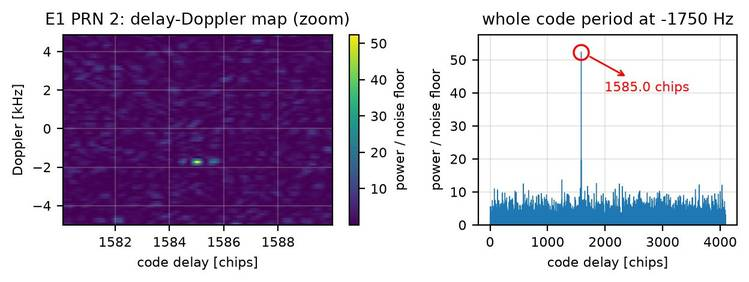
\includegraphics[width=1.0\linewidth]{gnss_sdr/x310_20261026T190001Z/galileo_acq_1B.jpg}
  \caption{Acquisition, E1: delay--Doppler search of PRN 2; one sharp peak (test statistic 73 vs threshold 52) at -1750~Hz and 1585.0~chips.}
\end{figure}

\begin{figure}[H]
  \centering
  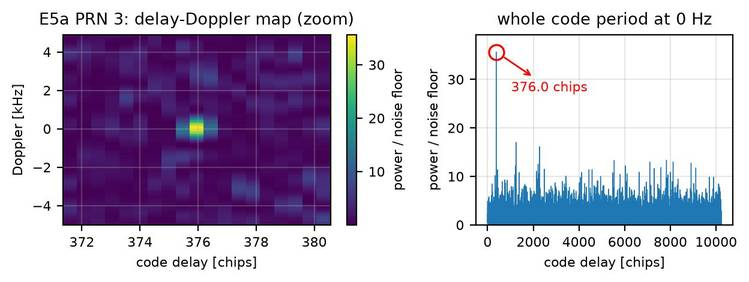
\includegraphics[width=1.0\linewidth]{gnss_sdr/x310_20261026T190001Z/galileo_acq_5X.jpg}
  \caption{Acquisition, E5a: delay--Doppler search of PRN 3; one sharp peak (test statistic 49 vs threshold 49) at 2223~Hz and 376.0~chips.}
\end{figure}

\begin{table}[H]
  \centering
  \footnotesize
  \resizebox{\ifdim\width>\linewidth\linewidth\else\width\fi}{!}{%
  \begin{tabular}{lrrrr}
    \hline
    \textbf{Band} & \textbf{Attempts} & \textbf{Detections} & \textbf{Detected PRNs} & \textbf{Best statistic / threshold\footnotemark} \\
    \hline
    E1 & 7 & 1 & 2 & 1.4 \\
    E5a & 74 & 1 & 3 & 1.0 \\
    \hline
  \end{tabular}}
  \caption{Acquisition: search attempts of the dumped channel. Attempts on satellites that are not in view (or do not broadcast that signal, e.g. older GPS satellites on L5/L2C) are rejected below the threshold.}
\end{table}

\footnotetext{Margin of the band's strongest detection: the largest acquisition test statistic among the detected attempts (the correlation peak of the delay--Doppler grid, normalised by the power of the input samples searched, i.e. the noise power, since GNSS signals are below the noise) divided by the detection threshold, which GNSS-SDR derives from the configured probability of false alarm. A value of 1 is right at the detection limit; e.g. 2.5 means the peak cleared the threshold 2.5 times over.}

\subsubsection{Tracking}


\begin{figure}[H]
  \centering
  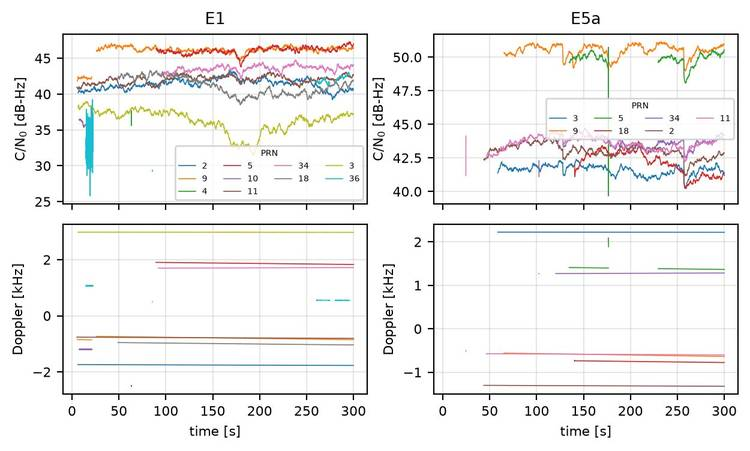
\includegraphics[width=1.0\linewidth]{gnss_sdr/x310_20261026T190001Z/galileo_tracking.jpg}
  \caption{Tracking: carrier-to-noise density ratio and carrier Doppler per satellite, while phase-locked (smooth Doppler curves = loops following the real satellite motion).}
\end{figure}

\begin{figure}[H]
  \centering
  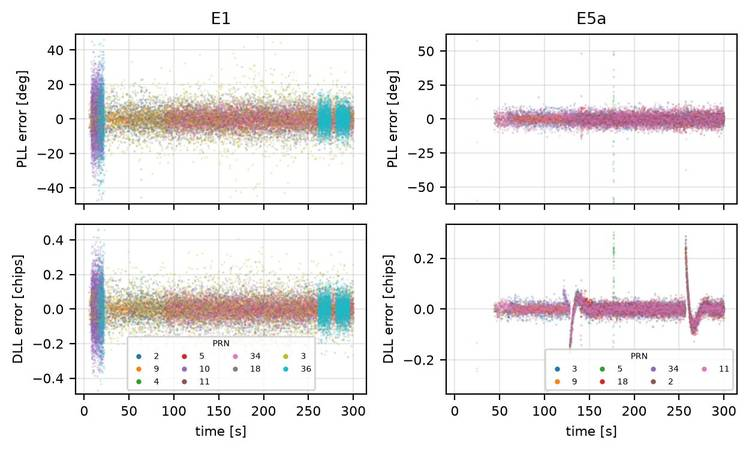
\includegraphics[width=1.0\linewidth]{gnss_sdr/x310_20261026T190001Z/galileo_tracking_errors.jpg}
  \caption{Tracking: loop errors per satellite while phase-locked, i.e. the discriminator outputs that the loops drive to zero: PLL carrier-phase error (degrees) and DLL code-delay error (chips) of every correlation. Noise centred on zero = clean tracking; its spread grows as C/N$_0$ drops, and jumps would mark cycle slips or a loop losing lock.}
\end{figure}

\begin{figure}[H]
  \centering
  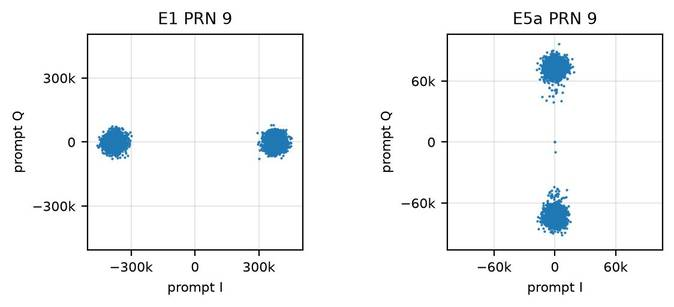
\includegraphics[width=1.0\linewidth]{gnss_sdr/x310_20261026T190001Z/galileo_tracking_iq.jpg}
  \caption{Tracking: prompt correlator outputs of the strongest satellite per band. Two tight clusters on one axis (the $\pm1$ data bits; GNSS-SDR's L5 tracking puts the data component on the Q axis), or, for the dataless pilots tracked for Galileo (E1-C, E5a-Q), the $\pm1$ chips of their secondary code, mean the PLL is phase-locked; a ring would mean it is not. \texttt{Prompt\_I}/\texttt{Prompt\_Q} are 32-bit floats (sums of the samples over one integration period, in file units): they never clip, only overflowing beyond $\pm 3.4\times10^{38}$, far above the $N\cdot\text{full scale}\cdot\sqrt{2}$ a sum of $N$ samples can reach.}
\end{figure}

\begin{table}[H]
  \centering
  \footnotesize
  \resizebox{\ifdim\width>\linewidth\linewidth\else\width\fi}{!}{%
  \begin{tabular}{lrrrrrrrr}
    \hline
    \textbf{Band} & \textbf{Ch.} & \textbf{PRN} & \textbf{Median C/N$_0$ [dB-Hz]} & \textbf{Phase-locked [\%]} & \textbf{Losses of lock} & \textbf{Tracked [s]} & \textbf{PLL error std [deg]} & \textbf{DLL error std [chips]} \\
    \hline
    E1 & 0 & 2 & 41.4 & 98 & 0 & 298 & 6.2 & 0.066 \\
    E1 & 1 & 9 & 46.2 & 97 & 1 & 300 & 3.3 & 0.037 \\
    E1 & 2 & 4 & 38.5 & 1 & 4 & 63 & 57.4 & 0.106 \\
    E1 & 2 & 5 & 46.1 & 98 & 4 & 216 & 3.6 & 0.040 \\
    E1 & 2 & 10 & 36.2 & 64 & 4 & 21 & 12.3 & 0.125 \\
    E1 & 3 & 11 & 42.1 & 98 & 0 & 300 & 6.1 & 0.062 \\
    E1 & 4 & 34 & 43.3 & 70 & 4 & 299 & 4.9 & 0.052 \\
    E1 & 5 & 18 & 41.0 & 84 & 2 & 299 & 6.5 & 0.071 \\
    E1 & 6 & 3 & 36.7 & 98 & 0 & 298 & 11.9 & 0.121 \\
    E1 & 7 & 36 & 44.5 & 12 & 14 & 299 & 9.2 & 0.089 \\
    E5a & 8 & 3 & 41.6 & 51 & 0 & 263 & 3.8 & 0.033 \\
    E5a & 9 & 9 & 50.7 & 50 & 0 & 258 & 1.4 & 0.027 \\
    E5a & 10 & 5 & 34.1 & 10 & 3 & 185 & 8.0 & 0.043 \\
    E5a & 11 & 18 & 42.1 & 42 & 0 & 171 & 4.4 & 0.033 \\
    E5a & 12 & 34 & 43.7 & 44 & 0 & 198 & 2.9 & 0.035 \\
    E5a & 13 & 2 & 42.8 & 53 & 0 & 275 & 3.2 & 0.029 \\
    E5a & 15 & 11 & 43.1 & 52 & 0 & 275 & 4.5 & 0.030 \\
    \hline
  \end{tabular}}
  \caption{Tracking: per channel and satellite (phase-locked: carrier lock test $> 0.8$; loop error standard deviations while phase-locked).}
\end{table}

\subsubsection{Telemetry decoder}


\begin{figure}[H]
  \centering
  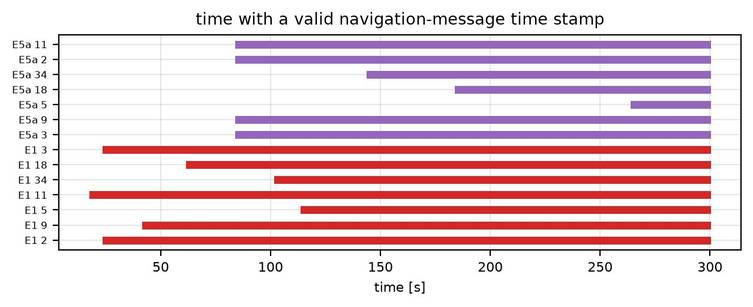
\includegraphics[width=1.0\linewidth]{gnss_sdr/x310_20261026T190001Z/galileo_telemetry.jpg}
  \caption{Telemetry decoder: per band and satellite, when the decoder delivered a valid transmit time (the first one comes after the first complete frame/message).}
\end{figure}

\begin{table}[H]
  \centering
  \footnotesize
  \resizebox{\ifdim\width>\linewidth\linewidth\else\width\fi}{!}{%
  \begin{tabular}{lrrrrr}
    \hline
    \textbf{Band} & \textbf{PRN} & \textbf{Messages decoded} & \textbf{Ephemeris} & \textbf{First valid at [s]} & \textbf{TOW [s]} \\
    \hline
    E1 & 2 & 27 & yes & 23.8 & 154850.0 \\
    E1 & 3 & 25 & yes & 23.8 & 154850.0 \\
    E1 & 5 & 18 & yes & 113.8 & 154940.0 \\
    E1 & 9 & 25 & yes & 41.8 & 154868.0 \\
    E1 & 11 & 27 & yes & 17.8 & 154844.0 \\
    E1 & 18 & 24 & yes & 61.8 & 154888.0 \\
    E1 & 34 & 19 & yes & 101.8 & 154928.0 \\
    E5a & 2 & 12 & yes & 84.1 & 154910.3 \\
    E5a & 3 & 12 & yes & 84.1 & 154910.3 \\
    E5a & 5 & 1 & yes & 264.0 & 155090.3 \\
    E5a & 9 & 12 & yes & 84.0 & 154910.3 \\
    E5a & 11 & 12 & yes & 84.0 & 154910.3 \\
    E5a & 18 & 4 & yes & 184.0 & 155010.3 \\
    E5a & 34 & 8 & yes & 144.1 & 154970.3 \\
    \hline
  \end{tabular}}
  \caption{Telemetry decoder: E1 I/NAV words, E5a F/NAV pages decoded, ephemeris obtained, and the first valid time of week.}
\end{table}

\subsubsection{Observables}
Pseudorange, carrier phase and Doppler of every channel at common receiver epochs.

\begin{figure}[H]
  \centering
  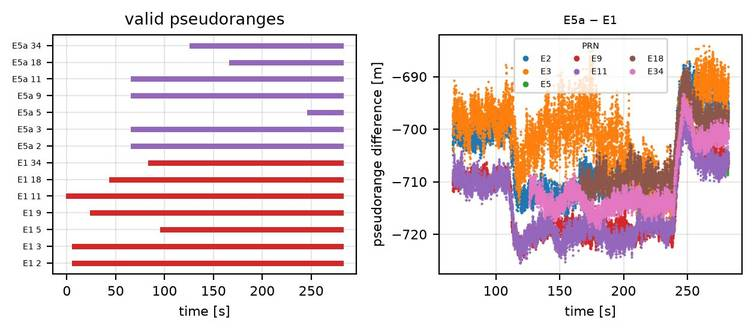
\includegraphics[width=1.0\linewidth]{gnss_sdr/x310_20261026T190001Z/galileo_observables.jpg}
  \caption{Observables: epochs with a valid pseudorange per band and satellite, and the difference between the two bands' pseudoranges of the same satellite (a constant receiver inter-band bias, the same for every satellite, plus the slowly varying ionospheric delay).}
\end{figure}

\begin{table}[H]
  \centering
  \footnotesize
  \resizebox{\ifdim\width>\linewidth\linewidth\else\width\fi}{!}{%
  \begin{tabular}{lrrrrrr}
    \hline
    \textbf{Difference} & \textbf{PRN} & \textbf{Common epochs} & \textbf{of run [\%]} & \textbf{Mean [m]} & \textbf{Std [m]} & \textbf{Drift [m/s]} \\
    \hline
    E5a $-$ E1 & 2 & 9649 & 64 & -705.48 & 7.29 & 0.0272 \\
    E5a $-$ E1 & 3 & 9649 & 64 & -700.47 & 6.77 & 0.0028 \\
    E5a $-$ E1 & 5 & 1769 & 12 & -703.48 & 2.96 & -0.2477 \\
    E5a $-$ E1 & 9 & 9649 & 64 & -714.02 & 6.79 & 0.0259 \\
    E5a $-$ E1 & 11 & 9649 & 64 & -714.54 & 6.51 & 0.0227 \\
    E5a $-$ E1 & 18 & 5271 & 35 & -704.75 & 6.76 & 0.1565 \\
    E5a $-$ E1 & 34 & 7027 & 47 & -710.08 & 6.21 & 0.0963 \\
    \hline
  \end{tabular}}
  \caption{Observables: pseudorange difference between the two bands of each satellite at common epochs (similar means = shared receiver bias; std = code noise of both bands).}
\end{table}

\subsubsection{PVT}
Position from the pseudoranges and the decoded ephemeris, compared with the surveyed antenna position (-23.209433$^\circ$, -45.874875$^\circ$, 596.42~m).

\begin{figure}[H]
  \centering
  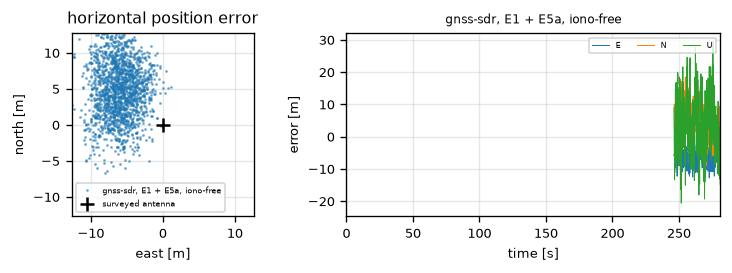
\includegraphics[width=1.0\linewidth]{gnss_sdr/x310_20261026T190001Z/galileo_pvt.jpg}
  \caption{PVT: position error of GNSS-SDR's own RTKLIB solution with respect to the surveyed antenna position.}
\end{figure}

\begin{table}[H]
  \centering
  \footnotesize
  \resizebox{\ifdim\width>\linewidth\linewidth\else\width\fi}{!}{%
  \begin{tabular}{l>{\centering\arraybackslash}p{4.2cm}}
    \hline
    \textbf{Solution} & \textbf{gnss-sdr, E1 + E5a, iono-free} \\
    \hline
    Solutions & 1732 \\
    Run with fix [\%] & 13 \\
    Mean E / N / U [m] & -6.0 / 4.9 / 3.0 \\
    Std E / N / U [m] & 2.3 / 4.1 / 8.1 \\
    RMS 2-D [m] & 9.0 \\
    RMS 3-D [m] & 12.5 \\
    95\% horiz. [m] & 13.7 \\
    \hline
  \end{tabular}}
  \caption{PVT: position error statistics with respect to the surveyed antenna (mean = accuracy, std = precision; \% of the run's seconds with a position; GNSS-SDR outputs several solutions per second).}
\end{table}

